\documentclass{article}
\usepackage{amsmath}
\usepackage{amssymb}
\usepackage{empheq}
\usepackage{hyperref}
\usepackage[most]{tcolorbox}
\usepackage{verbatim}
\usepackage{pgfplots}
\usepackage{pgf,tikz}
\usepackage{geometry}
\geometry{a4paper, total={170mm,257mm},
           left=20mm, top=20mm }

\usetikzlibrary{positioning, patterns}
\usetikzlibrary{decorations.pathmorphing}
\usetikzlibrary{arrows.meta, shadows, shapes.symbols}
\graphicspath{ {./images/} }
%%\pgfplotsset{compat=1.15}

\begin{document}

\title{On determination of function extrema with MaxEnt formulation}
\author{Ravi Sankar Saripalli}

\maketitle

\begin{tcolorbox}[fonttitle=\sffamily\bfseries\large,
                  title=Description]

                  This is an attempt to find extrema of a function 
                  with MaxEnt formulation. The usual way to
                  find extrema of a function $f(x)$  is to find $x$ where function
                  derivative $f^\prime (x)$ vanishes. An alternate approach is to use probability distribution function
                  $p(x)$ as an independant parameteric function and seek to maximize the expected value of $f(x)$ based on the
                  $p(x)$ with the condition that entropy (as defined by Shanon) of the probability distribution $p(x)$ is maximized, thus
                  ensuring that the distribution function derived is least biased.

\end{tcolorbox}
\begin{tcolorbox}[fonttitle=\sffamily\bfseries\large,
                  title=The MaxEnt Lagrangian]

%% Equation 1
\begin{empheq}[box=\tcbhighmath]{equation}
  \begin{split}
       \mathcal{L} (p, \lambda ) = \int f(x) p(x) dx 
                                    + T  \int p(x) ln(p(x)) dx 
                                    + \lambda \left \{ \left ( \int p(x) dx \right ) - 1 \right \}  
  \end{split}
\end{empheq}

    The first term in the Lagrangian is the expected value of the function corresponding to the PDF $p(x)$,
    the second term corresponds
    to the entropy of the PDF scaled by an arbitray constant $T$ and the last  term corresponds to the equality 
    constraint that integral of PDF is one. The multiplier $\lambda$ is the Lagrangian parameter.
\\
    Noting that the Lagrangian is function of $p(x)$ and $\lambda$,  the extrema of the Lagrangian is obtained
    by requiring the functional derivative with respect $p(x)$ and the Lagrangian parameter $\lambda$ are zero.
    
    Although this enables us to determine $p(x)$ and $\lambda$ corresponding to the extrema, we need additional
    criterion to determine if the extrema is either 
    minimum or maximum. Whether one can use the sign of the  second derivative in functional space 
    similar to simple variables can be used for this purpose is yet to be explored by me....

    Also, what role the scaling multiplier $T$ on the entropy function in the overall objective is not very clear
    to me.
\end{tcolorbox}

\begin{tcolorbox}[fonttitle=\sffamily\bfseries\large,
                  title=The Euler-Lagrange equation]

Consider the following functional (function of functions)
%% Equation 2
\begin{empheq}[box=\tcbhighmath]{equation}
  \begin{split}
      & F \left( f^{\prime}, f, x \right) = \int \phi \left ( f^{\prime} (x), f(x), x \right) dx  
  \end{split}
\end{empheq}

  Requiring that functional derivative of $F$ with respect to $f$ is zero at extrema  
 (note $f$ is a function not a variable, hence 
   the name functional derivative) following Eauler-Lagrange  equation can be derived.

%% Equation 3
\begin{empheq}[box=\tcbhighmath]{equation}
       \frac{\partial \phi}{\partial y}
          - \frac{d}{dx}\left( \frac{\partial \phi}{\partial y^\prime} \right) = 0 
\end{empheq}
    \text{Derivation of the above equation that is easy to follow is  
    \href{https://farside.ph.utexas.edu/teaching/336L/Fluid/node266.html}{here}}

\end{tcolorbox}


\begin{tcolorbox}[fonttitle=\sffamily\bfseries\large,
                  title=Finding Stationary Point of Lagrangian in Eq 1.]

Using the above Euler-Lagrange equation, the stationary conditions for the Lagrangian in equation 1, 
can be derived from functional derivative with respective $p$ and the 
derivative with respective $\lambda$ as follows.

%%Equation 4
\begin{empheq}[box=\tcbhighmath]{equation}
  \begin{split}
      & f(x) + T \left\{ 1  + ln(p(x)) \right\} + \lambda = 0
  \end{split}
\end{empheq}

%%Equation 5
Setting derivative with respect to $\lambda$ to zero yields the contraint that PDF integral should be 1.
\begin{empheq}[box=\tcbhighmath]{equation}
  \begin{split}
      & \int p(x) \:  dx  - 1 = 0  
  \end{split}
\end{empheq}

%%Equation 6
Rearranging eqn.4 
\begin{empheq}[box=\tcbhighmath]{equation}
  \begin{split}
      &  p(x) =  e^{ -\left( 1 + \lambda / T  \right) }   \: e^{-f(x)/T}
  \end{split}
\end{empheq}

Combining eqns. 5 and 6 the value of lambda can be expressed as follows
\begin{empheq}[box=\tcbhighmath]{equation}
  \begin{split}
      &  \lambda = T \left\{ ln \int e^{-f(x)/T} dx  - 1 \right\}
  \end{split}
\end{empheq}

    The question to ask is how do we now proceed to get min or max of $f(x)$ given that we have it
    in analytical form (eg. sin(x)).. What will be the p(x) as T approaches zero. That is the intent
    of the annealing process as we converge on p(x).
\end{tcolorbox}

\begin{tcolorbox}[fonttitle=\sffamily\bfseries\large,
                   title=Explorations with sinx ]
  Assuming that we are interested in finding extrema of sin(x) in the interval $[0,\pi]$,
  one can proceed as follows.
  \begin{enumerate}
     \item {For a given T, calculate $\lambda$ by evaluating the integral numerically}
     \item {With $T and \lambda$ known, the PDF $p(x)$ now is well defined (eq.6). The expected value of $f(x)$ can be
       determined by numerical integration of $\int p(x) f(x) dx$ }
  \end{enumerate}
 
\end{tcolorbox}

\begin{tcolorbox}[fonttitle=\sffamily\bfseries\large,
  title={$sin(x)$} ]
    \centering
     %% Generates x) plot between 0 and pi
  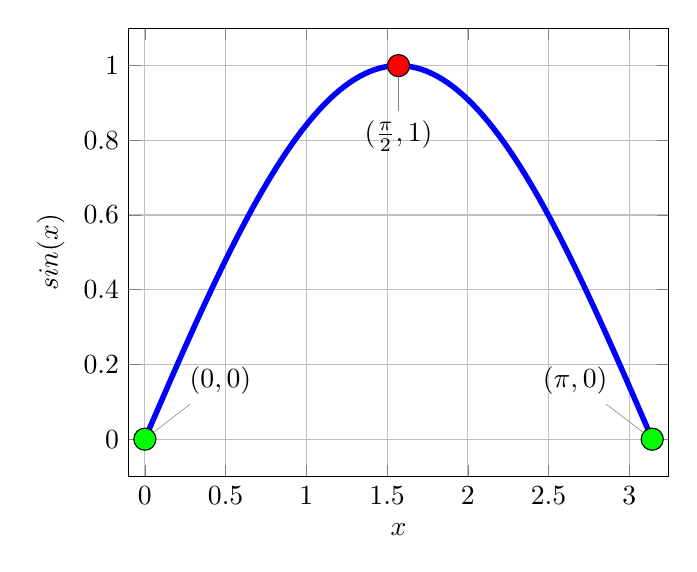
\begin{tikzpicture}
    \begin{axis}[ xlabel = $x$,
	  ylabel = {$sin(x)$},
	  ymin = -0.1, ymax = 1.1,
	  xmin = -0.1, xmax = pi + 0.1,
	  grid=both,
	  domain = 0:pi
	]
       \addplot[color=blue, line width=2pt, samples=100] 
          {sin(x*180/pi)} ;
       \addplot[only marks, mark options={fill=green,scale=2} ]
          coordinates { (0,0) (pi, 0) } ;
       \addplot[only marks, mark options={fill=red,scale=2} ]
	  coordinates { (pi/2, 1) };
	  
	  \node[pin=270:{$(\frac{\pi}{2}, 1)$}] at (axis cs:pi/2,1) {} ;
	  \node[pin=45:{$(0,0)$}] at (axis cs:0,0) {} ;
	  \node[pin=135:{$(\pi,0)$}] at (axis cs:pi,0) {} ;
    \end{axis}
  \end{tikzpicture}

\end{tcolorbox}

\begin{tcolorbox}[fonttitle=\sffamily\bfseries\large,
  title={Change in pdf with T when $T \le 0$ and $T \ge 0$} ]
     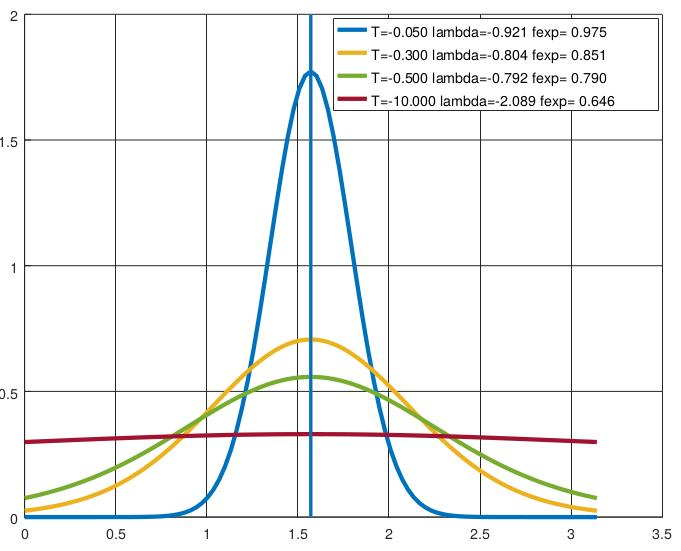
\includegraphics[scale=0.25]{fig1.jpg}
     \hspace{1cm}
     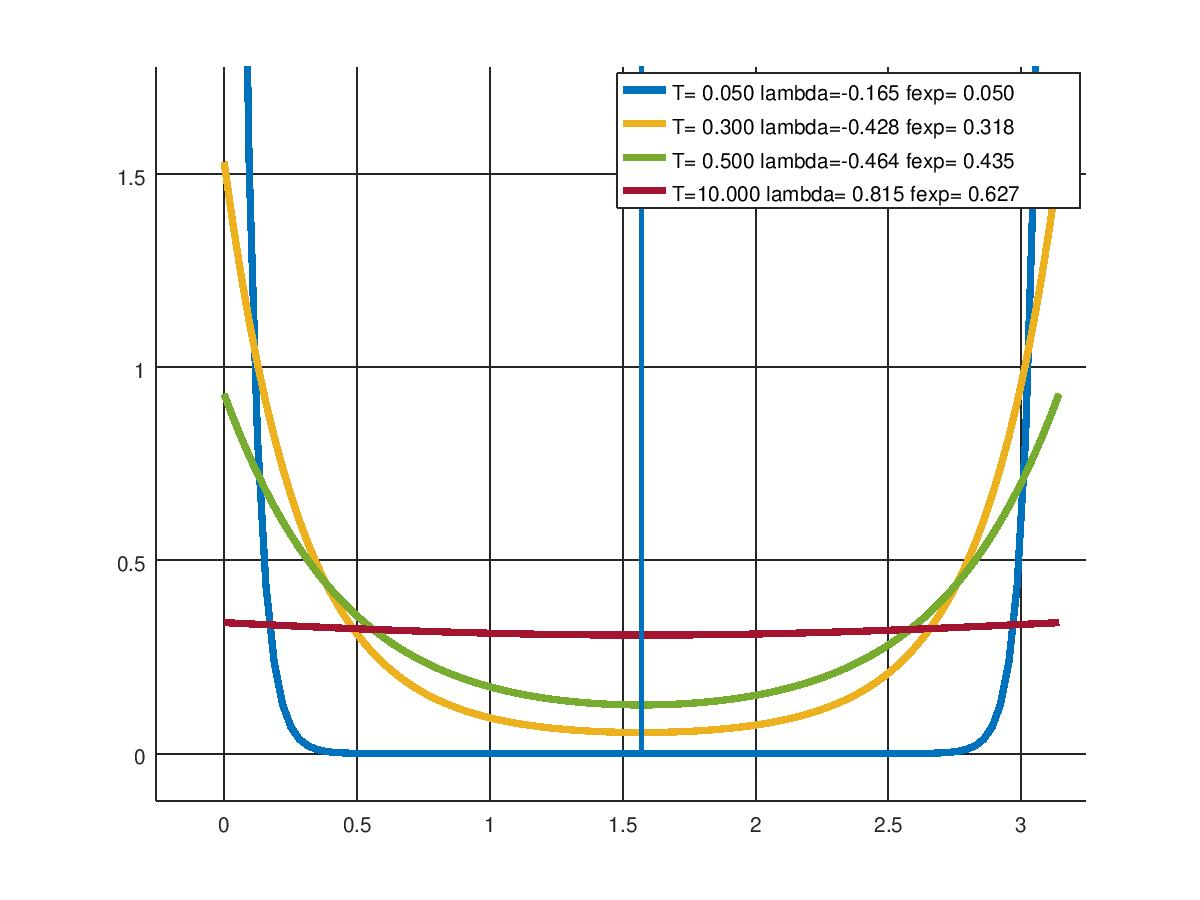
\includegraphics[scale=0.32]{fig2.jpg}
\end{tcolorbox}


From the above figures, it is clear that for $T \ge 0$ as its 
magnitude approaches zero, the pdf spread decreases and
tends to peak around the true maxima. On the otherhand,
when $T \ge 0$, the pdf peaks appear near the end points where
the function has minimal value in the interval of interest. 

Let us now explore a different function that has two peaks, and trough as shown in the
following figure. 
\begin{tcolorbox}[fonttitle=\sffamily\bfseries\large,
    title={$y(x)=8(1-2x^2)x^2  -0.6<x<0.6  $} ]
    \centering
     %% Generate 8*(1-2*x^2)*x^2
%%  between x=-0.6 to 0.6

  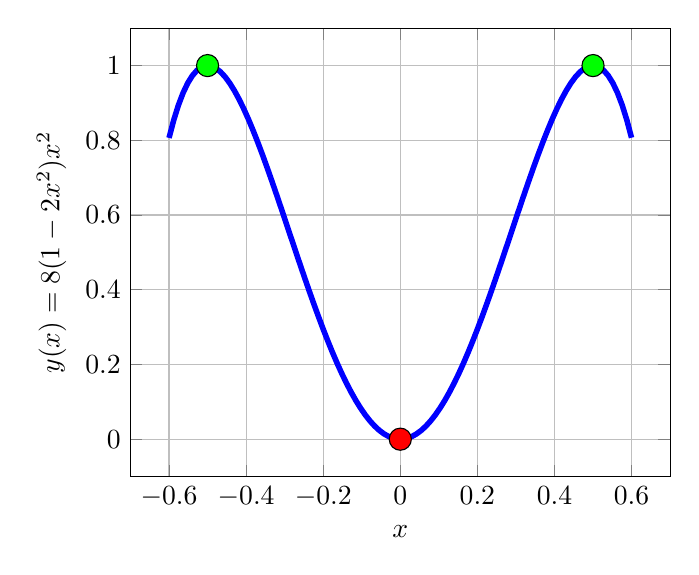
\begin{tikzpicture}
    \begin{axis}[ xlabel = $x$,
        ylabel = {$y(x)=8(1-2x^2)x^2$},
	  ymin = -0.1, ymax = 1.1,
	  xmin = -0.7, xmax = 0.7,
	  grid=both,
	  domain = -0.6:0.6
	]
       \addplot[color=blue, line width=2pt, samples=100] 
	  {8*(1-2*x*x)*x*x)} ;
          
       \addplot[only marks, mark options={fill=green,scale=2} ]
          coordinates { (-0.5, 1) (0.5, 1) } ;
       \addplot[only marks, mark options={fill=red,scale=2} ]
	  coordinates { (0,0) };
	  
	  
    \end{axis}
  \end{tikzpicture}

\end{tcolorbox}

Using the above function, the effect of $T$ on PDF corresponding to the stationary
point is determined as described earlier.

\begin{tcolorbox}[fonttitle=\sffamily\bfseries\large,
    title={Effect of $T$ on PDF at stationary condition}  ]
     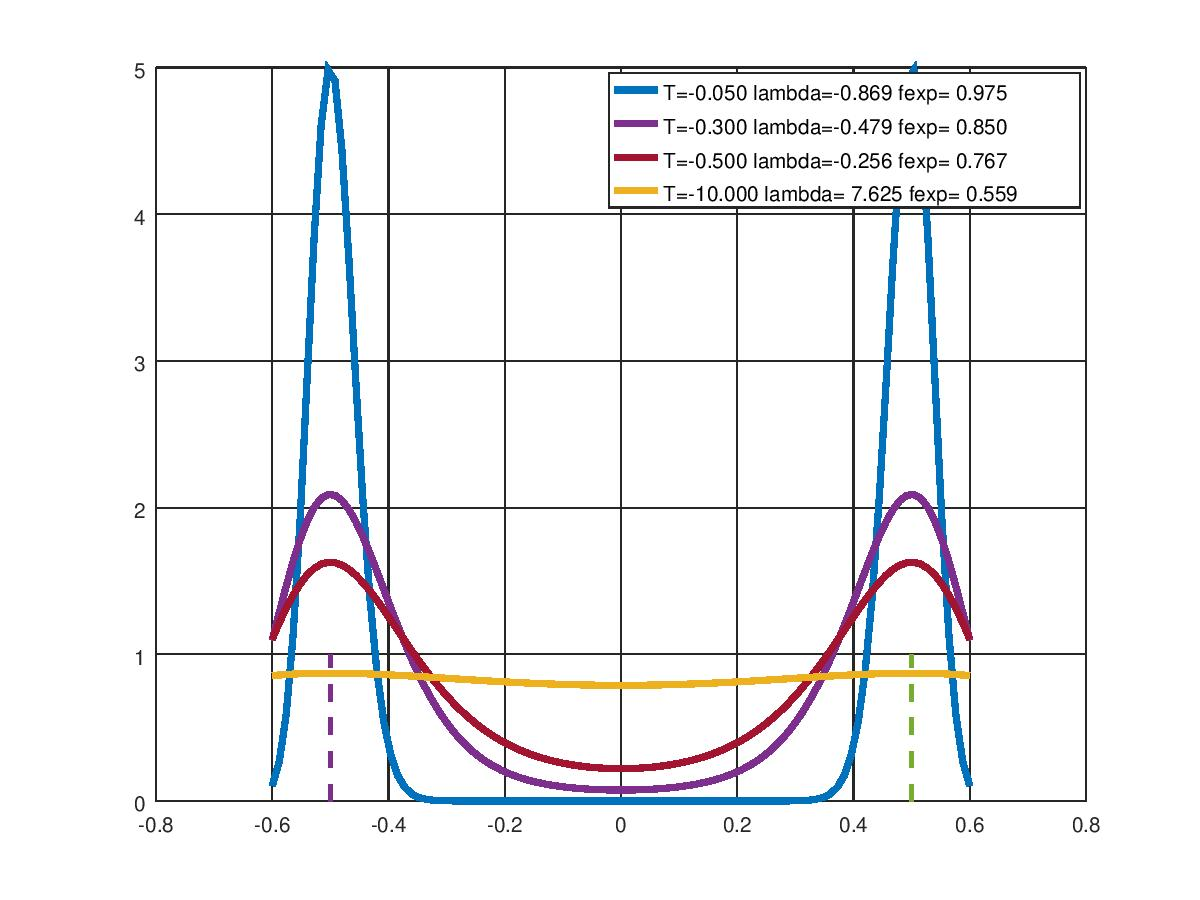
\includegraphics[scale=0.3]{fig3.jpg}
     \hspace{1cm}
     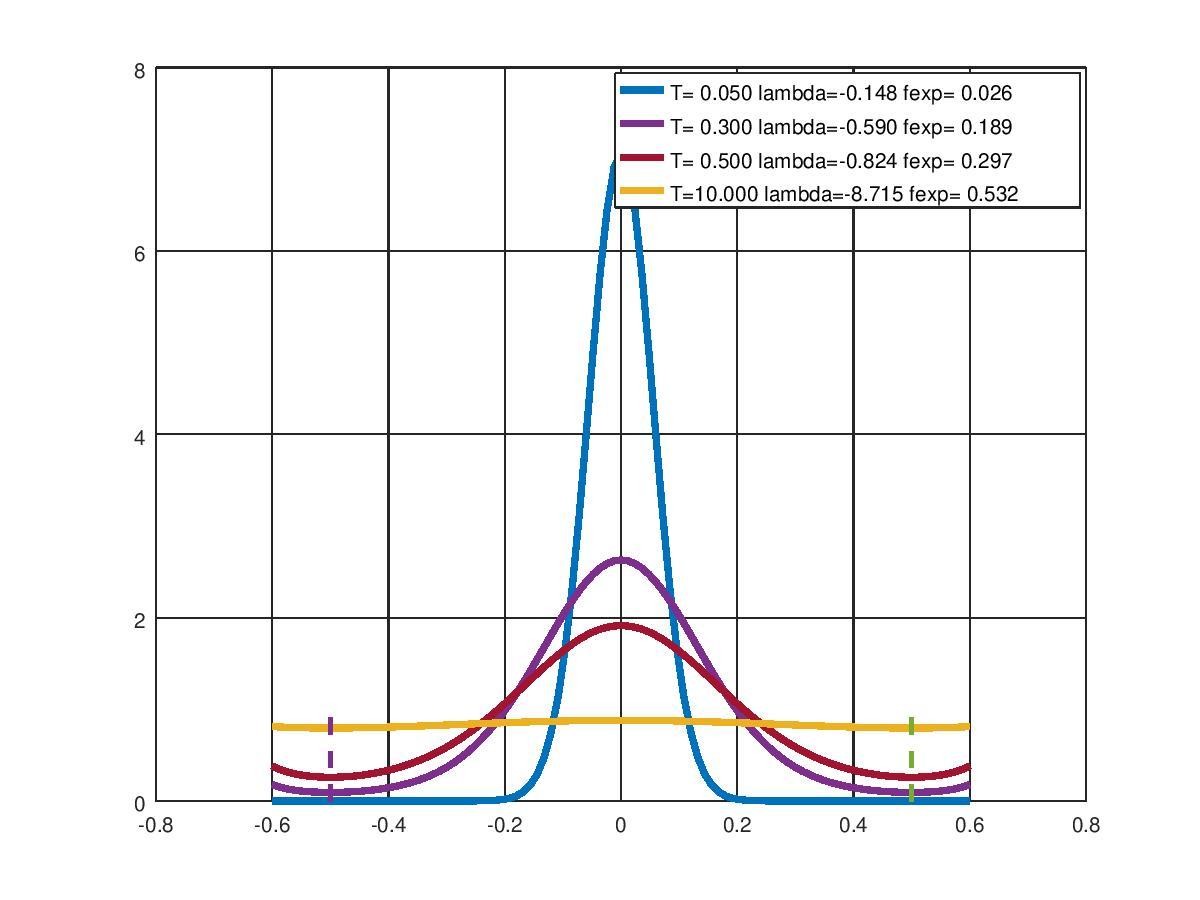
\includegraphics[scale=0.3]{fig4.jpg}
\end{tcolorbox}

Once again, when $T$ value is approaching zero from positive side,
the PDF corresponding to extrema condition peaks around the true minima
at $x=0$ with corresponding expected value of function approaching 0.
When $T$ approaches zero from the negative side, the PDF peaks around
$x=-0.5, and 0.5$ with expected value of function approaching 1.

It therefore appears that when $T$ approaches zero from negative side
PDF determined from stationary condition corresponds to maxima of the function,
while it approaches zero from positive side, the PDF peaks around the minima of the 
function.


\end{document}
